\section{Approach}
\label{sec:appr}

This section describes problems related to \unsafe{} that we identified, as well as information on how to exploit these issues in the wild.
Furthermore, we present our two novel tools, \toolUsage{} and \toolSA{}, that aid in locating, evaluating and fixing potentially dangerous \unsafe{} usages.


%% ---------------------------------------------------

\subsection{Usage and Security Problems}
\label{sec:appr:vulnerabilites}

In the following, we discuss potential threat models and exploit vectors against real-world \unsafe{} Go code.
We present a code pattern in Listing~\ref{lst:string-to-bytes} that is very common in popular open-source Go projects (cf. Section~\ref{sec:eval}).
It is used to convert a string to a byte slice without copying the data.
As in Go strings essentially are just read-only byte slices, this is commonly done by projects to increase efficiency of serialization operations. % and is possible as in Go, strings are essentially read-only byte slices.
Internally, each slice is represented by a data structure that contains its current length, allocated capacity, and memory address of the actual underlying data array.
The \textit{reflect} header structures provide access to this internal representation.
In Listing~\ref{lst:string-to-bytes} this conversion is done in line 2, 3, and 8 respectively.
First, an \textit{unsafe.Pointer} is used to convert a string to a \textit{reflect.StringHeader} type.
Then, a \textit{reflect.SliceHeader} instance is created and its fields are filled by copying the respective values from the string header.
Finally, the slice header object is converted into a slice of type \textit{[]byte}.

\begin{lstlisting}[language=Golang, label=lst:string-to-bytes, caption=Conversion from string to bytes using \unsafe{}, float, belowskip=-1.5em]
func StringToBytes(s string) []byte {
	strHeader := (*reflect.StringHeader)(unsafe.Pointer(&s))
	bytesHeader := reflect.SliceHeader{
		Data: strHeader.Data,
		Cap:  strHeader.Len,
		Len:  strHeader.Len,
	}
	return *(*[]byte)(unsafe.Pointer(&bytesHeader))
}
\end{lstlisting}


\subsubsection*{Implicit Read-Only}

The conversion pattern shown in Listing~\ref{lst:string-to-bytes} is efficient as it directly casts between \textit{string} and \textit{[]byte} in-place. %, without the need to reallocate the slice.
Using \textit{bytes := ([]byte)(s)} for the conversion would make the compiler allocate new memory for the slice header as well as the underlying data array.
However, the direct cast creates an implicitly read-only byte slice that can cause problems, as described in the following.
The Go compiler will place strings into a constant data section of the resulting binary file.
Therefore, when the binary is loaded into memory, the \textit{Data} field of the string header may contain an address that is located on a read-only memory page.
Hence, strings in Go are immutable by design and mutating a string causes a compiler error. %, alerting developers early in the development process that there is a problem.
However, when casting a string to a \textit{[]byte} slice in-place, the resulting slice loses the explicit read-only property, and thus, the compiler will not complain about mutating this slice although the program will crash if done so.
%Using this pattern, therefore, creates a trade-off between performance and potentially hard-to-find bugs that can lead to crashes.
%Due to the indirection resulting from the conversion to a slice which gets then passed around, they can be very hard to debug.


\subsubsection*{Garbage Collector Race}

Go uses a concurrent mark-and-sweep \textit{garbage collector (GC)} to free unused memory~\cite{sibiryov2017}.
It is triggered either by a certain increase of heap memory usage or after a fixed time. %, and runs in multiple parallel threads (Goroutines).
The GC treats pointer types, \textit{unsafe.Pointer} values, and slice/string headers as references and will mark them as still in use. %, preventing them from being freed.
Importantly, string/slice headers that are created manually as well as \textit{uintptr} values are not treated as references.
The last point, although documented in the \textit{unsafe} package, is a major pitfall.
Casting an \textit{uintptr} variable back to a pointer type creates a potentially dangling pointer because the memory at that address might have already been freed if the GC was triggered right before the conversion.

Although not directly obvious, Listing~\ref{lst:string-to-bytes} contains such a condition.
Because the \textit{reflect.SliceHeader} value is created as a composite literal instead of being derived from an actual slice value, its \textit{Data} field is not treated as a reference if the GC runs between lines 3 and 8. 
Thus, the underlying data array of the \textit{[]byte} slice produced by the conversion might have already been collected.
This creates a potential \textit{use-after-free} or buffer reuse condition that, even worse, is triggered non-deterministically when the GC runs at just the "right" time.
%If the buffer is reused after being freed and the slice resulting from the cast is pointing to it, it can provide access to completely unrelated data. % even in concurrent Goroutines. 
Therefore, this race condition can crash the program, create an information leak, or even potentially lead to code execution.
Figure~\ref{fig:gcrace-vuln} shows a visualization of the casting process that leads to the problems described here.
The original slice is being cast to a string via some intermediate representations.
The slice header is shown in green (at memory position 1), while the underlying data array (memory position 2) is shown in red.
When the resulting string header (shown in blue at memory position 3) is created, it only has a weak reference to the data, and when the GC runs before converting it to the final string value, the data is already freed.

\begin{figure}[!t]
    \vspace{2mm}
    \centering
    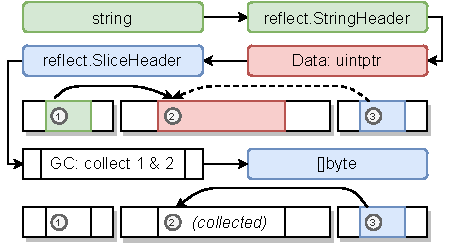
\includegraphics[width=0.4\textwidth]{gfx/figures/gcrace-vuln.pdf}
    %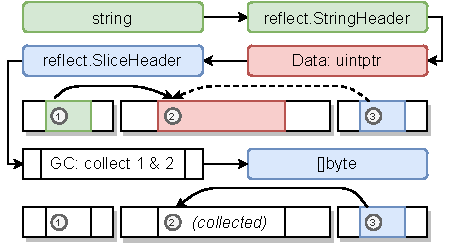
\includegraphics[width=0.48\textwidth]{gfx/figures/gcrace-vuln.pdf}
    \caption{GC race and escape analysis flaw}
    \label{fig:gcrace-vuln}
    \vspace{-8pt}
\end{figure}



\subsubsection*{Escape Analysis Flaw}

A third problem found in Listing~\ref{lst:string-to-bytes} is that the \textit{escape analysis (EA)} algorithm can not infer a connection between the string parameter \textit{s} and the resulting byte slice.
Although, they use the same underlying data array, the EA misses this due to the fact that the intermediate representation as a \textit{uintptr} is not treated as a reference type.
This can cause undefined behavior if the returned value from the casting function is used incorrectly.

Listing~\ref{lst:escape-analysis} shows a program that uses the conversion function presented earlier~(Listing~\ref{lst:string-to-bytes}).
In the \textit{main} function, \textit{GetBytes} is called~(Line 2), which creates a string and turns it into a byte slice using the conversion function.
Within the \textit{GetBytes} function, we create the string using a \textit{bufio} reader similarly to if it were user-provided input.
After the cast, \textit{GetBytes} prints the resulting bytes~(Line 10) and returns them to \textit{main}, which also prints the bytes~(Line~3).
Although, one might assume that both print statements result in the same string to be displayed, the second one in \textit{main} fails and prints invalid data.


% // expected (but failed) stdout is "abcdefgh
% // expected stdout is "abcdefgh"
\begin{lstlisting}[language=Golang, label=lst:escape-analysis, caption=Escape analysis flaw example, float, belowskip=-1.5em]
func main() {
	bytesResult := GetBytes()
	fmt.Printf("main: %s\n", bytesResult)
}

func GetBytes() []byte {
	reader := bufio.NewReader(strings.NewReader("abcdefgh"))
	s, _ := reader.ReadString('\n')
	out := StringToBytes(s)
	fmt.Printf("GetBytes: %s\n", out)
	return out
}
\end{lstlisting}

\begin{figure}[htp!]
    %\vspace{2mm}
    \centering
    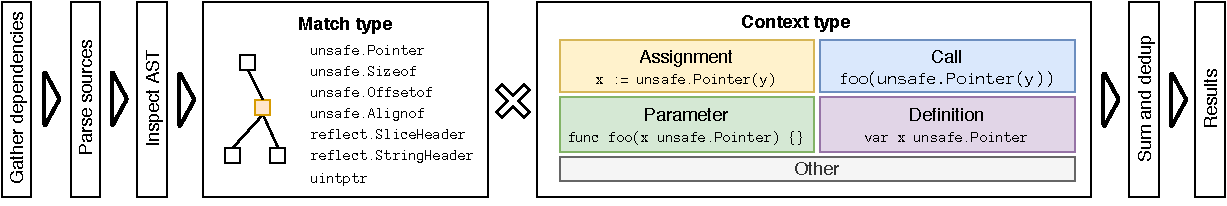
\includegraphics[width=\textwidth]{assets/figures/chapter4/go-geiger-architecture.pdf}
    \caption{Architecture of the \toolGeiger{} tool to detect unsafe usages}
    \label{fig:geiger-architecture}
    %\vspace{-10pt}
\end{figure}


Because the string \textit{s} is allocated in \textit{GetBytes} the Go escape analysis is triggered. %try to figure out if it escapes.
It concludes that \textit{s} is passed to \textit{StringToBytes} and the EA transitively looks into that function.
Here, it fails to connect \textit{s} to the returned byte slice as described previously.
Therefore, the EA concludes that \textit{s} does not escape in \textit{StringToBytes}.
As it is not used after the call in \textit{GetBytes}, the EA algorithm incorrectly assumes that it does not escape at all and places \textit{s} on the stack.
When \textit{GetBytes} prints the resulting slice, the data is still valid and the correct data is printed, but once the function returns to \textit{main}, its stack is destroyed.
Thus, \textit{bytesResult} (Line~2) is now a dangling pointer into the former stack of \textit{GetBytes} and, therefore, printing data from an invalid memory region.


%\subsubsection*{Correct In-Place Cast}
%
%To avoid the problems described in the previous sections, it is crucial to not create instances of \textit{reflect.SliceHeader} and \textit{reflect.StringHeader} from scratch, instead they must be derived from actual slices or strings.
%Although this is documented with the \textit{unsafe} package, there are many incorrect usages in the projects we analyzed.
%A correct version of the in-place cast is shown in Listing~\ref{lst:correct-slice-cast}.
%
%\begin{lstlisting}[language=Golang, label=lst:correct-slice-cast, caption=Correct in-place string to bytes cast]
%func StringToBytes(s string) (b []byte) {
%	strHeader := (*reflect.StringHeader)(unsafe.Pointer(&s))
%	bytesHeader := (*reflect.SliceHeader)(unsafe.Pointer(&b))
%	bytesHeader.Data = strHeader.Data
%	bytesHeader.Cap = strHeader.Len
 %   bytesHeader.Len = strHeader.Len
%	return
%}
%\end{lstlisting}


\subsubsection*{Code Execution}

To show the severity of the issues identified above and that they are not just of theoretical nature, e.g., resulting in simple program crashes, we created a proof of concept for a code execution exploit using \textit{Return Oriented Programming (ROP)} on a vulnerable \unsafe{} usage. %vulnerability caused by a misuse of \unsafe{}.
The sample incorrectly casts an array on the stack into a slice without constricting it to the proper length.
This vulnerability causes a buffer overflow which we use to overwrite the stored return address on the stack, thus, changing the control flow of the program. 
Since Go programs are typically statically linked with a big runtime, there is a large number of ROP-gadgets available within the binary itself. 
We use gadgets to set register values and dispatch to system calls. 
Using the \textit{mprotect} syscall, we set both the writable and executable permission bits on a memory page that is mapped to the program, and store an exploit payload on that page using the \textit{read} syscall. Finally, we jump to this payload as if it were our last ROP gadget, executing it and opening a shell.
An in-depth discussion of the exploit would go beyond the scope of this paper and exceed the space available to present our research.
Therefore, we made it available online\footnote{\url{https://github.com/jlauinger/go-unsafepointer-poc}\label{fn:poc}} together with five other proof-of-concepts. 



%% ---------------------------------------------------


\subsection{\toolUsage{}: Identification of Unsafe Usage}

This section presents \toolUsage{}, a novel tool to identify and quantify usages of \unsafe{} in a package and in its dependencies, which is available on GitHub\footnote{\url{https://github.com/jlauinger/go-geiger}}.
Its development was inspired by \textit{cargo geiger}\footnote{\url{https://github.com/rust-secure-code/cargo-geiger}}, a similar tool for detecting unsafe code blocks in Rust programs.

%\subsubsection*{Approach}

Figure~\ref{fig:geiger-architecture} shows an overview of the architecture of \toolUsage{}.
We use the standard parsing infrastructure provided by Go to identify and parse packages including their dependencies based on user input.
%In particular, we use the \textit{packages.Load} function to parse the sources of all packages requested for analysis including their transitive dependencies.
Then, we analyze the AST, %using the standard \textit{ast.Inspect} function.
which enables us to identify different usages of \unsafe{} and their context as described in the next paragraph.
Finally, we arrange the packages requested for analysis and their dependencies in a tree structure, sum up \unsafe{} usages for each package individually, and calculate a cumulative score including dependencies.
We perform a deduplication if the same package is transitively imported more than once.
The \unsafe{} dependency tree, usage counts, as well as identified code snippets, are presented to the user.

%\subsubsection*{Implementation}

We detect all usages of methods and fields from the \textit{unsafe} package, specifically: \textit{Pointer}, \textit{Sizeof}, \textit{Offsetof}, and \textit{Alignof}.
Furthermore, because they often are used in unsafe operations, we also count occurrences of \textit{SliceHeader} \textit{StringHeader} from the \textit{reflect} package, and \textit{uintptr}.
All of these usages are referred to as \unsafe{} usages in this paper.
%The first six \unsafe{} types are detected by finding selector expression nodes with matching field names, while \textit{uintptr} usages are found by inspecting identifier nodes in the AST.
Additionally, we determine the context in which the \unsafe{} usage is found, i.e., 
the type of statement that includes the \unsafe{} usage.
In \toolUsage{} we distinguish between assignments (including definitions of composite literals and return statements), calls to functions, function parameter declarations, general variable definitions, or other not further specified usages.
We determine the context by looking up in the AST starting from the node representing the \unsafe{} usage, and identifying the type of the parent node.
%For example, if the nearest relevant ancestor in the AST is an \textit{AssignStmt} node, then the context is determined as assignment.

%% ---------------------------------------------------



\subsection{\toolSA{}: An Unsafe-focused Linter}

%This section presents \toolSA{}, a novel static code analysis tool to find dangerous \unsafe{} usage patterns that were previously uncaught with existing tools. 
Through the usage of \toolUsage{} in real-world code and our manual analysis, we found \unsafe{} code patterns that were not covered by existing linters such as \textit{go vet}. 
To automatically give advice for these patterns we designed \toolSA{}.
It is meant for assistance during manual audits and also for integration in build chains during development.
All source code for \toolSA{} is made publicly available\footnote{\url{https://github.com/jlauinger/go-safer}}.
Avoiding the \unsafe{} usage patterns that \toolSA{} warns about prevents the garbage collector race and escape analysis flaw vulnerabilities that we discussed in Section~\ref{sec:appr:vulnerabilites}.

%\subsubsection*{Approach}

\begin{figure}[!t]
    \vspace{2mm}
    \centering
    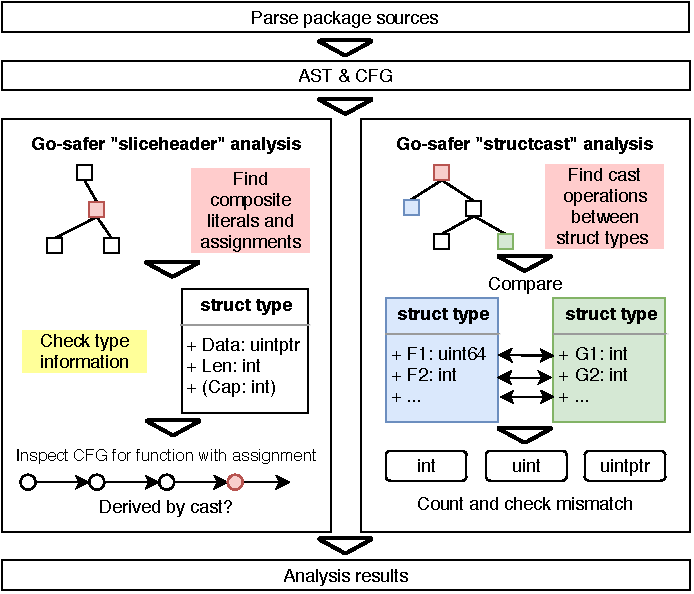
\includegraphics[width=0.48\textwidth]{gfx/figures/go-safer-architecture.pdf}
    %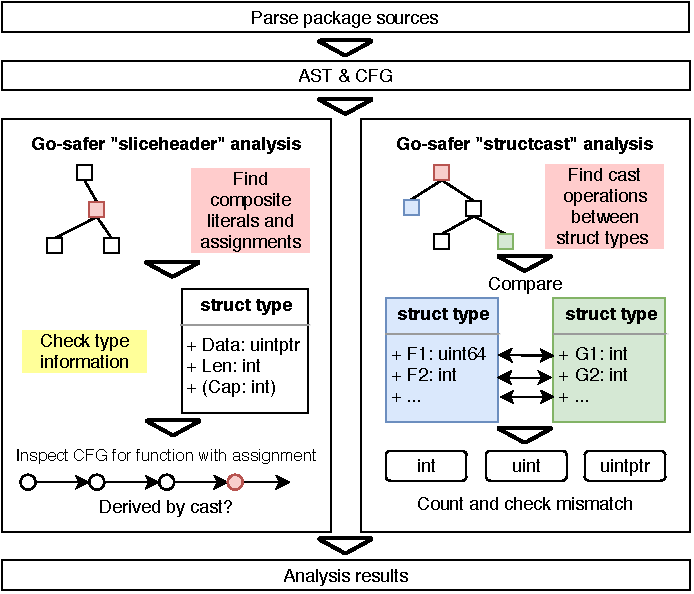
\includegraphics[width=0.45\textwidth]{gfx/figures/go-safer-architecture.pdf}
    \caption{Architecture of \toolSA{} static code analysis tool}
    \label{fig:safer-architecture}
    %\vspace{-14pt}
\end{figure}


Figure~\ref{fig:safer-architecture} shows an overview of the architecture of \toolSA{}.
%It was built on top of the existing infrastructure provided by the \textit{go vet} tool.
First, it uses \textit{go vet} to build a list of packages to be analyzed and parses their sources.
Then, a number of static code analyzers, called \textit{passes}, run.
Our analyses depend on existing passes to acquire the abstract syntax tree (AST) and control flow graph (CFG).
\toolSA{} runs two separate analyses: the \textit{sliceheader} and the \textit{structcast} passes. % discovers incorrect string and slice casts as shown in Listing~\ref{lst:string-to-bytes}.
%The \textit{structcast} pass finds unsafe casts between different struct types that include architecture-dependent field sizes and, therefore, might create a security risk when ported to other platforms.
%Describing potential exploit vectors for this second type of problem is beyond the scope of this paper, thus, we added an example of this to the public repository\textsuperscript{\ref{fn:poc}} mentioned in the last section.

%\subsubsection*{Implementation}

The \textit{sliceheader} pass discovers incorrect string and slice casts as shown in Listing~\ref{lst:string-to-bytes}.
It finds composite literals and assignments in the AST.
Then, for each it checks whether the type of the %literal or assignment 
receiver is \textit{reflect.StringHeader}, \textit{reflect.SliceHeader}, or some derived type with the same signature.
For assignments, the analysis pass then finds the last node in the CFG where the receiver object's value is defined, and checks if it is derived correctly by casting a string/slice.
If we can not infer with certainty that the assignment receiver object was created by a cast, then \toolSA{} issues a warning.

The \textit{structcast} pass discovers instances of in-place casts between different struct types that include architecture-dependent field sizes. 
This can create a security risk when ported to other platforms because \unsafe{} casts can lead to misaligned fields, and thus, memory access outside a value's bounds on some platforms, allowing the same exploit vectors as a buffer overflow does.
The pass finds struct cast instances that involve \textit{unsafe.Pointer} in the AST.
Then, it compares the struct types and checks if they contain an unequal amount of fields with types \textit{int}, \textit{uint}, or \textit{uintptr}, which are the architecture-dependent types supported by Go.
If the numbers do not match, \toolSA{} issues a warning.

